\documentclass[a4paper,11pt]{article}

\usepackage[a4paper,left=2.5cm,right=2.5cm,top=3.5cm,bottom=3.5cm]{geometry}
\usepackage[utf8]{inputenc}
\usepackage[T1]{fontenc}
\usepackage[english]{babel}
\usepackage{graphicx}
\usepackage{amsmath,amssymb,amsthm,amsopn}
\usepackage{mathrsfs}
\usepackage{graphicx}
\usepackage{array}
\usepackage{makecell}
\usepackage{bm}
\usepackage{hyperref}
\usepackage[shortlabels]{enumitem}
\hypersetup{
    colorlinks=true,
    linkcolor=blue,
    citecolor=red,
}
\usepackage{diagbox}

\usepackage{algorithm}
\usepackage{algpseudocode}

\renewcommand{\algorithmicrequire}{\textbf{Input:}}
\renewcommand{\algorithmicensure}{\textbf{Output:}}

%\usepackage[top=1cm,bottom=1cm]{geometry}
%\usepackage{listings}
%\usepackage{xcolor}

\usepackage{tikz}
\usetikzlibrary{arrows}

% Tikz style

\tikzset{round/.style={circle, draw=black, very thick, scale = 0.7}}
\tikzset{arrow/.style={->, >=latex}}
\tikzset{dashed-arrow/.style={->, >=latex, dashed}}

\newtheoremstyle{break}%
{}{}%
{\itshape}{}%
{\bfseries}{}%  % Note that final punctuation is omitted.
{\newline}{}

\newtheoremstyle{sc}%
{}{}%
{}{}%
{\scshape}{}%  % Note that final punctuation is omitted.
{\newline}{}

\theoremstyle{break}
\newtheorem{thm}{Theorem}[section]
\newtheorem{lm}[thm]{Lemma}
\newtheorem{prop}[thm]{Proposition}
\newtheorem{cor}[thm]{Corollary}

\theoremstyle{sc}
\newtheorem{exo}{Exercice}

\theoremstyle{definition}
\newtheorem{defi}[thm]{Definition}
\newtheorem{ex}[thm]{Example}

\theoremstyle{remark}
\newtheorem{rem}[thm]{Remark}

% Math Operators

\DeclareMathOperator{\Card}{Card}
\DeclareMathOperator{\Gal}{Gal}
\DeclareMathOperator{\Id}{Id}
\DeclareMathOperator{\Img}{Im}
\DeclareMathOperator{\Ker}{Ker}
\DeclareMathOperator{\Minpoly}{Minpoly}
\DeclareMathOperator{\Mod}{mod}
\DeclareMathOperator{\Ord}{Ord}
\DeclareMathOperator{\ppcm}{ppcm}
\DeclareMathOperator{\tr}{Tr}
\DeclareMathOperator{\Vect}{Vect}
\DeclareMathOperator{\Span}{Span}
\DeclareMathOperator{\rank}{rank}
\DeclareMathOperator{\ev}{ev}

% Shortcuts

\newcommand{\dE}{\partial(E)}
\newcommand{\dF}{\partial(F)}
\newcommand{\dG}{\partial(G)}
\newcommand{\diff}{\mathop{}\!\mathrm{d}}
\newcommand{\eg}{\emph{e.g. }}
\newcommand{\emb}{\hookrightarrow}
\newcommand{\embed}[2]{\phi_{#1\hookrightarrow#2}}
\newcommand{\ent}[2]{[\![#1,#2]\!]}
\newcommand{\ie}{\emph{i.e. }}
\newcommand{\ps}[2]{\left\langle#1,#2\right\rangle}
\newcommand{\eqdef}{\overset{\text{def}}{=}}
\newcommand{\f}{f}%{\mathfrak{f}}
\newcommand{\bff}{\mathbf{f}}
\newcommand{\E}{\mathcal{E}}
\newcommand{\A}{\mathcal{A}}
\newcommand{\B}{\mathcal{B}}
\newcommand{\R}{\mathcal{R}}
\newcommand{\bfa}{\mathbf{a}}
\newcommand{\bfb}{\mathbf{b}}
\newcommand{\D}{\mathcal{D}}
\newcommand{\Pcal}{\mathcal{P}}
\newcommand{\musym}{\mu^{\textrm{sym}}}
\newcommand{\mutri}{\mu^{\textrm{tri}}}
\newcommand{\muhyp}{\mu^{\textrm{hyp}}}
\newcommand{\musymG}[1][G]{\mu^{\textrm{sym},#1}}
\newcommand{\mutriG}[1][G]{\mu^{\textrm{tri},#1}}
\newcommand{\muhypG}[1][G]{\mu^{\textrm{hyp},#1}}
\newcommand{\hmusym}{\hat\mu^{\textrm{sym}}}
\newcommand{\hmutri}{\hat\mu^{\textrm{tri}}}
\newcommand{\hmuhyp}{\hat\mu^{\textrm{hyp}}}
\newcommand{\hmusymG}[1][G]{\hat\mu^{\textrm{sym},#1}}
\newcommand{\hmutriG}[1][G]{\hat\mu^{\textrm{tri},#1}}
\newcommand{\hmuhypG}[1][G]{\hat\mu^{\textrm{hyp},#1}}
\newcommand{\Msym}{M^{\textrm{sym}}}
\newcommand{\Mtri}{M^{\textrm{tri}}}
\newcommand{\Mhyp}{M^{\textrm{hyp}}}
\newcommand{\hMsym}{\hat{M}^{\textrm{sym}}}
\newcommand{\hMtri}{\hat{M}^{\textrm{tri}}}
\newcommand{\hMhyp}{\hat{M}^{\textrm{hyp}}}
\newcommand{\tri}[2]{\mu_{#1}^{\text{tri}}(#2)}
\newcommand{\sym}[2]{\mu_{#1}^{m_3}(#2)}
\newcommand{\K}{\mathbf{k}}


% opening
\title{Asymptotic length of tri-symmetric formulas}
\author{}



\begin{document}

\maketitle

\begin{abstract}
In this notes we prove that the asymptotic length of a tri-symmetric
decomposition in $\mathbb{F}_{q^k}/\mathbb{F}_q$ is \emph{linear} in $k$, \ie is in $O(k)$.
We do not provide a thorough presentation of the background nor the interest
that such decompositions have. In order to have some of these elements, the
reader may want to look at~\cite{BDEZ12, Covanov18, Covanov19}.
\end{abstract}

%\tableofcontents

%\clearpage

\section{Introduction}
\label{sec:intro}

\paragraph{Definitions.} Let $\tr$ be the trace of the field extension
$\mathbb{F}_{q^k}/\mathbb{F}_q$, for any $x, y\in\mathbb{F}_{q^k}$, we let
\[
  \ps{x}{y} = \tr(xy),
\]
and if
\[
  \Phi:(\mathbb{F}_{q^k})^m\to\mathbb{F}_{q^k}
\]
is a $m$-linear map (over $\mathbb{F}_q$), then we say that we have a
$m$-symmetric decomposition of $\Phi$ if there exist $n$ elements
$a_i\in\mathbb{F}_{q^k}$ and $n$ elements $b_i\in\mathbb{F}_{q^k}$ such that
\[
  \forall (x_1, \dots, x_n)\in(\mathbb{F}_{q^k})^n,\,\Phi(x_1, \dots, x_n) =
  \sum_{i=1}^n\ps{a_i}{x_1}\dots\ps{a_i}{x_n}b_i.
\]
We only write \emph{symmetric} instead of $2$-symmetric. The same definition
applies for $m$-linear forms by replacing $\mathbb{F}_{q^k}$ by $\mathbb{F}_q$.
We say that we have a \emph{tri-symmetric} decomposition of a
$\mathbb{F}_{q}$-bilinear map
\[
  \Psi:\mathbb{F}_{q^k}\times\mathbb{F}_{q^k}\to\mathbb{F}_{q^k}
\]
is there exist $n$ elements $a_i\in\mathbb{F}_{q^k}$ and $n$ scalars
$\lambda_i\in\mathbb{F}_q$ such that
\[
  \forall x, y\in\mathbb{F}_{q^k},\,\Psi(x, y) =
  \sum_{i=1}^{n}\lambda_i\ps{a_i}{x}\ps{a_i}{y}a_i.
\]

\paragraph{Decompositions.} For any elements $x,y\in\mathbb{F}_{q^k}$, let
\[
m_2(x, y) = xy
\]
and
\[
t_2(x, y) = \tr(xy).
\]
Similarly, for any elements $x, y, z\in\mathbb{F}_{q^k}$, let
\[
m_3(x, y, z) = xyz
\]
and
\[
t_3(x, y, z) = \tr(xyz).
\]
In fact, having a tri-symmetric decomposition of $m_2$ is equivalent to having a
$3$-symmetric decomposition of the $3$-linear form $t_3$, as stated in Lemma~\ref{lm:m2t3}.
\begin{lm}
  \label{lm:m2t3}
  Let $n\in\mathbb{N}$ be a natural integer and for $1\leq i \leq n$, let
  $a_i\in\mathbb{F}_{q^k}$ and $\lambda_i\in\mathbb{F}_q$, then
  \[
    \forall x, y\in\mathbb{F}_{q^k},\, xy =
    \sum_{i=1}^n\lambda_i\ps{a_i}{x}\ps{a_i}{y}a_i
  \]
  if and only if
  \[
    \forall x, y, z\in\mathbb{F}_{q^k},\,\tr(xyz) =
    \sum_{i=1}^n\lambda_i\ps{a_i}{x}\ps{a_i}{y}\ps{a_i}{z}
  \]
\end{lm}
\begin{proof}
  In one direction, multiply by $z$ and take the trace. In the other, it follows
  from the fact that the trace is non degenerate.
\end{proof}

The question of the existence of tri-symmetric decompositions is treated
in~\cite{Randriam15}, but now we would like to have some bound on the
length $n$ of a tri-symmetric decomposition. More precisely, we want to show
that the length is a linear function of $k$. We only want to prove that the
length is linear and we do not make much effort to get the smallest possible
constants during the process. Recall that a tri-symmetric decomposition of $m_2$
is the same as a $3$-symmetric decomposition of $t_3$, using
Lemma~\ref{lm:m2t3}. The next lemma gives us a way of obtaining a $3$-symmetric decomposition of
$t_3$.
\begin{lm}
  Given a $3$-symmetric decomposition of $m_3$, one can deduce a $3$-symmetric
  decomposition of $t_3$.
\end{lm}
\begin{proof}
  Assume that there exist $n$ elements $a_i\in\mathbb{F}_{q^k}$ and $n$ elements
  $d_i\in\mathbb{F}_{q^k}$ with
  \[
    \forall x, y, z\in\mathbb{F}_{q^k},\,xyz =
    \sum_{i=1}^n\ps{a_i}{x}\ps{a_i}{y}\ps{a_i}{z}d_i.
  \]
  Then taking the trace, we obtain
  \[
    \tr(xyz) = \sum_{i=1}^n\tr(d_i)\ps{a_i}{x}\ps{a_i}{y}\ps{a_i}{z},
  \]
  that is exactly a $3$-symmetric decomposition of the $3$-linear form $t_3$.
\end{proof}
\begin{rem}
  We emphasize that this is probably not the optimal way of obtaining a
  $3$-symmetric decomposition of $t_3$.
\end{rem}
\paragraph{Notations.} We let $\tri{q}{k}$ be the tri-symmetric
bilinear complexity of $\mathbb{F}_{q^{k}}/\mathbb{F}_{q}$, \ie the minimal length $n$
of a tri-symmetric decomposition of the product in the extension
$\mathbb{F}_{q^k}/\mathbb{F}_q$. We let
$\sym{q}{k}$ be the minimal length $n$ of a $m$-symmetric decomposition of 
\[
  m_3:\mathbb{F}_{q^{k}}\times\mathbb{F}_{q^k}\times\mathbb{F}_{q^k}\to\mathbb{F}_{q^k}.
\].

\section{Evaluation-interpolation method}
\label{sec:eval}

Albeit not optimal, our strategy will be to find $3$-symmetric decomposition of
$m_3$ by an evaluation interpolation method. We use the function field
terminology and notations
presented in~\cite{Stichtenoth09}. Let $F/\mathbb{F}_q$ be an algebraic
function field of one variable over $\mathbb{F}_{q}$ and let $\mathbb{P}_F$ be the
set of places of $F$. Let $\D_F$ the set of
divisors on $F$, and if $D\in\D_F$ is a divisor on
$F$, we denote by $L(D)$ its Riemann-Roch space. The following proposition
highlights the method.

\begin{prop}
  \label{prop:method}
  Assume there exist a place $Q\in\mathbb{P}_{F}$ of $F$ of degree $k$, $P_1,
  \dots, P_n\in\mathbb{P}_F$ places of $F$ of degree $1$, and a divisor
  $D\in\D_F$ of $F$ such that the places $Q$ and $P_1, \dots, P_n$ are not in
  the support of $D$ and such the following conditions hold.
  \begin{enumerate}
    \item \label{cond:1} The evaluation map 
      \[
        \begin{array}{cccc}
        \ev_{Q, D}: & L(D) & \to & \mathbb{F}_{q^k}\\
  & f & \mapsto & f(Q)
\end{array}
\]
is \emph{surjective}.
    \item \label{cond:2} The evaluation map
      \[
        \begin{array}{cccc}
        \ev_{\Pcal, 3D}: & L(3D) & \to & (\mathbb{F}_{q})^n\\
  & h & \mapsto & (h(P_1), \dots, h(P_n))
\end{array}
\]
is \emph{injective}.
  \end{enumerate}
  Then we can compute a $3$-symmetric decomposition of $m_3$ of length $n$.
\end{prop}
\begin{proof}
  Since the map $\ev_{Q, D}$ is surjective, it admits a right inverse $s$, \ie a
  map 
  \[
        \begin{array}{cccc}
          s: & \mathbb{F}_{q^k} & \to & L(D)
\end{array}
  \]
  such that
  \[
    \ev_{Q, D}\circ s = \Id_{\mathbb{F}_{q^k}},
  \]
  where $\Id_{\mathbb{F}_{q^k}}$ is the identity map on $\mathbb{F}_{q^k}$, and
  for all $x\in\mathbb{F}_{q^k}$, we denote $s(x)\in L(D)$ by $f_x$. We
  also let
  \[
        \begin{array}{cccc}
          a: & \mathbb{F}_{q^k} & \to & (\mathbb{F}_{q})^n \\
          & x & \mapsto & (f_x(P_1), \dots, f_x(P_n))
\end{array}
  \]
  be the map $a = \ev_{\Pcal, D}\circ s$. The situation is sumed up in the
  following drawing.
   \begin{center}
  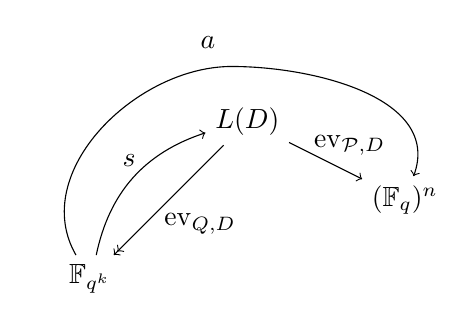
\begin{tikzpicture}
    \node (LD) at (2, 2) {$L(D)$};
    \node (Fqk) at (0, 0) {$\mathbb{F}_{q^k}$};
    \node (Fqn) at (4, 1) {$(\mathbb{F}_{q})^n$};
    \draw[->>] (LD) to (Fqk);
    \draw[->] (LD) to (Fqn);
    \draw[->] (Fqk) to[bend left] (LD);
    \node (s) at (0.5, 1.5) {$s$};
    \node (evQ) at (1.4, .7) {$\ev_{Q, D}$};
    \node (evP) at (3.3, 1.7) {$\ev_{\Pcal, D}$};
    \draw[->] (Fqk) to[out=120,in=180](1.8, 2.7) to[out=0, in=70] (Fqn);
    \node (a) at (1.5, 3) {$a$};
  \end{tikzpicture}
  \end{center}
  For all $1\leq i\leq n$, the map
  $x\mapsto f_x(P_i)$ is a linear form, so there exists an element
  $a_i\in\mathbb{F}_{q^k}$ such that
  \[
    \forall x\in\mathbb{F}_{q^k},\, f_x(P_i) = \ps{a_i}{x},
  \]
  thus
  \[
    \forall x\in\mathbb{F}_{q^k},\, a(x) = (\ps{a_1}{x}, \dots, \ps{a_n}{x}).
  \]
  Let $x, y, z\in\mathbb{F}_{q^k}$, and
  \[
    p = a(x)*a(y)*a(z)\in(\mathbb{F}_{q})^n
  \]
  be the coordinate-wise product of the elements $a(x)$, $a(y)$, and $a(z)$. In
  other words, 
  \[
    p = (f_xf_yf_z(P_1), \dots, f_xf_yf_z(P_n)).
  \]
  Similarly, since the map $\ev_{\Pcal, 3D}$ is injective, it admits a left inverse $r$, \ie a
  map 
  \[
        \begin{array}{cccc}
          r: & (\mathbb{F}_{q})^n & \to & L(D)
\end{array}
  \]
  such that
  \[
    r\circ\ev_{\Pcal, 3D} = \Id_{L(D)},
  \]
  where $\Id_{L(D)}$ is the identity map on $L(D)$. We
  also let
  \[
        \begin{array}{cccc}
          d: & (\mathbb{F}_{q})^n & \to & \mathbb{F}_{q^k} \\
\end{array}
  \]
  be the map $d = \ev_{Q, 3D}\circ r$.   The situation is sumed up in the
  following drawing.
  \begin{center}
  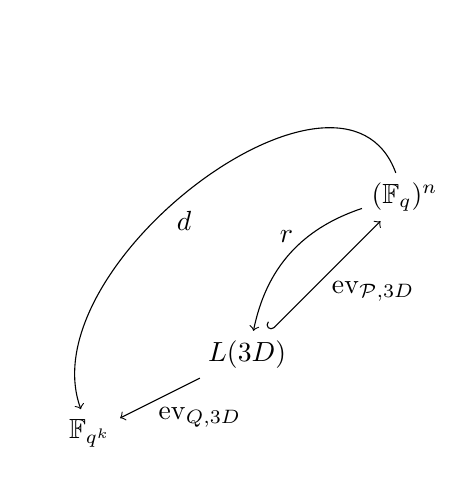
\begin{tikzpicture}
    \node (L3D) at (2, 1) {$L(3D)$};
    \node (Fqk) at (0, 0) {$\mathbb{F}_{q^k}$};
    \node (Fqn) at (4, 3) {$(\mathbb{F}_{q})^n$};
    \draw[right hook->] (L3D) to (Fqn);
    \draw[->] (L3D) to (Fqk);
    \draw[->] (Fqn) to[bend right] (L3D);
    \node (evP) at (3.6, 1.8) {$\ev_{\Pcal, 3D}$};
    \node (s) at (2.5, 2.5) {$r$};
    \node (evQ) at (1.4, .2) {$\ev_{Q, 3D}$};
    \draw[->] (Fqn) to[out=110,in=110] (Fqk);
    \node (d) at (1.2, 2.7) {$d$};
  \end{tikzpicture}
\end{center}
The map $r$ is linear on
  $\Img(\ev_{\Pcal, 3D})$, so $d$ is also linear on $\Img(\ev_{\Pcal, 3D})$, by
  composition of two linear maps. Thus we have $n$ elements $d_1, \dots, d_n$ of
  $\mathbb{F}_{q^k}$ such that, for all $(x_1, \dots, x_n)\in\Img(\ev_{\Pcal,
  3D})$, 
  \[
    d(x_1, \dots, x_n) = \sum_{i=1}^n x_i d_i.
  \]
Now 
\[
  h = r(p)\in L(3D)
\]
is an element of $L(3D)$ such that
\[
  \forall 1\leq i\leq n,\,\ev_{\Pcal, 3D}(h) = f_xf_yf_z(P_i), 
\]
but this is also the case for the function $f_xf_yf_z\in L(3D)$. Since the map
$\ev_{\Pcal, 3D}$ is injective, we have 
\[
  h = f_xf_yf_z.
\]
Then, we have 
\begin{equation*}
  \begin{split}
  d(p) &= \ev_{Q, 3D}(r(p))\\
  &= \ev_{Q, 3D}(h)\\
  &= h(Q)\\
  &= f_x(Q)f_y(Q)f_z(Q)\\
  &= s(x)(Q)s(y)(Q)s(z)(Q)\\
  &= \ev_{Q, D}\circ s(x)\ev_{Q, D}\circ s(y)\ev_{Q, D}\circ s(z)\\
  &= xyz.
  \end{split}
\end{equation*}
But we also have 
\begin{equation*}
  \begin{split}
    p &= a(x)*a(y)*a(z)\\
    &= (\ps{a_1}{x}\ps{a_1}{y}\ps{a_1}{z}, \dots,
    \ps{a_n}{x}\ps{a_n}{y}\ps{a_n}{z}),
  \end{split}
\end{equation*}
so 
\[
  d(p) = \sum_{i=1}^n\ps{a_i}{x}\ps{a_i}{y}\ps{a_i}{z}d_i
\]
and finally we have a $3$-symmetric decomposition of $m_3$:
\[
  xyz = \sum_{i=1}^n\ps{a_i}{x}\ps{a_i}{y}\ps{a_i}{z}d_i.
\]
\end{proof}
Now that we know the method to find $3$-symmetric decompositions of $m_3$, and thus
tri-symmetric decompositions of $m_2$, the question is, given $q$ and $k$, to
find an algebraic function field $F/\mathbb{F}_{q}$ satisfying
Proposition~\ref{prop:method}. If $F/\mathbb{F}_q$ is a function field of genus
$g$ and $G\in\D_F$ a divisor of $F$, Riemann's theorem states that
\[
  \dim L(G) \geq \deg G + 1 - g,
\]
with equality if $\deg G > 2g - 2$. Assume that there exist $Q\in\mathbb{P}_F$ a
place of $F$ of degree $k$, $P_1, \dots, P_n$ places of degree $1$ and
$D\in\D_F$ a divisor which support does not include $Q, P_1, \dots, P_n$. Since 
\[
  \Ker(\ev_{\Pcal, 3D}:L(3D)\to(\mathbb{F}_{q})^n) = L(3D-P_1-\dots-P_n),
\]
the injectivity in Condition~\eqref{cond:2} is equivalent to
\[
  L(3D-P_1-\dots-P_n)=\left\{ 0 \right\}.
\]
This is the case if
\[
\deg(3D-P_1-\dots-P_n)<0,
\]
which is the case if
\[
  n > 3\deg D.
\]
Similarly, we have
\[
  \Ker(\ev_{Q, D}:L(D)\to\mathbb{F}_{q^k}) = L(D-Q),
\]
and the rank-nullity theorem states that
\[
  \dim L(D) = \dim\Ker(\ev_{Q, D})+\dim\Img(\ev_{Q, D}),
\]
so the surjectivity in Condition~\eqref{cond:1} is equivalent to
\[
  \dim L(D-Q) = \dim L(D) - k.
\]
A sufficient condition for the last equation to hold is that
\[
  \deg D > k+ 2g - 2,
\]
because
\begin{equation*}
  \begin{split}
  \deg(D-Q) &= \deg D - \deg Q\\
  &= \deg D - k\\
  &> 2g - 2
  \end{split}
\end{equation*}
and so 
\begin{equation*}
  \begin{split}
    \dim L(D-Q) &= \deg(D-Q)+1-g\\
    &=\deg D+1-g-k\\
    &=\dim L(D)-k.
  \end{split}
\end{equation*}
Thus, a sufficient condition for Conditions~\eqref{cond:1} and~\eqref{cond:2} to
hold is that
\[
  \frac{n}{3} > \deg D > k + 2g - 2.
\]
If $\frac{n}{3}>k + 2g -1$, there exists an integer $\delta\in\mathbb{N}$ with
\[
  \frac{n}{3} > \delta > k +2g -2,
\]
\eg $\delta=k+2g-1$, therefore we can assume without loss of generality that there
exists a divisor $D$ of degree $\delta$ which support does not include $Q, P_1,
\dots, P_n$, thanks to the strong approximation theorem.

The remaining part is to prove that we can find suitable function fields for
each $q$ fixed and $k\to\infty$. It means that we look for a function field
$F/\mathbb{F}_q$ of genus $g$, with a place of degree $k$, and such that there
are at least $n$ places of degree $1$, with
\[
  n > 3k +6g - 3
\]
in order to apply Proposition~\ref{prop:method}. Let us start with the special case of $q\geq64$
a square. In this case, we know~\cite{STV92} that there exists a family of function fields
$F_i/\mathbb{F}_q$ of genus $g_i$ such that
\begin{enumerate}
  \item $g_i\to\infty$
  \item $\frac{g_{i+1}}{g_i}\to1$
  \item $N_i\sim (\sqrt q - 1)g_i$
\end{enumerate}
with
\[
  N_i = \Card\left\{ P\in\mathbb{P}_{F_i}\,|\,\deg P = 1 \right\}
\]
the number of places of degree $1$ of $F_i$. We also assume that the sequence
$(g_i)_i$ is increasing. For each $k$, let $g_{i(k)}$ be the
smallest genus $g_i$ such that
\[
  N_{i} > 3k + 6g_{i}.
\]
This is always possible to find such an index $i(k)$ since 
\[
  N_i\sim (\sqrt q - 1)g_i
\]
and $\sqrt q -1 > 6$. By definition, we thus have
\[
  N_{i(k)-1}\leq 3k+6g_{i(k)-1}<3k+6g_{i(k)}<N_{i(k)}.
\]
Since $i(k)\to\infty$ when $k\to\infty$, we can use the asymptotic results on the
family of function fields $F_i$, so we know
\begin{equation*}
  \begin{split}
  N_{i(k)-1} &\sim (\sqrt q-1)g_{i(k)-1}\\
  &\sim (\sqrt q-1)g_{i(k)}\\
  &= (\sqrt q-1)g_{i(k)}+o(g_{i(k)}).
  \end{split}
\end{equation*}
Similarly, 
\[
  N_{i(k)} = (\sqrt q -1)g_{i(k)}+o(g_{i(k)}),
\]
and so we deduce that
\begin{equation}
  3k = (\sqrt q -7)g_{i(k)} + o(g_{i(k)})
  \label{eqn:equivg}
\end{equation}
and
\begin{equation}
  g_{i(k)}= \frac{3}{\sqrt q - 7}k+o(k).
  \label{equivk}
\end{equation}
We know~\cite[Corollary 5.2.10.]{Stichtenoth09} there exists a place of degree
$k$ in $F_{i(k)}$ if we have
\begin{equation}
  2g_{i(k)} +1 \leq q^{(k-1)/2}(\sqrt q-1),
  \label{eqn:degreek}
\end{equation}
but thanks to Equation~\eqref{eqn:equivg} we know that
Inequation~\eqref{eqn:degreek} is true as soon as $k$ is large enough. Let
$k_0(q)$ be a constant such that~\eqref{eqn:degreek} is true for $k\geq k_0(q)$.
If $q\geq 64$ is a square and $k\geq k_0(q)$, we now know that we can find a
function field $\mathbb{F}_{i(k)}$ in which Proposition~\ref{prop:method}
applies, so that we can find a $3$-symmetric decomposition of $m_3$ of length
$n$, and therefore a tri-symmetric decomposition $\mathbb{F}_{q^k}/\mathbb{F}_q$ of length $n$, with
\begin{equation*}
  \begin{split}
    n&\leq N_{i(k)}\\
    &= (\sqrt q -1)g_{i(k)}+o(g_{i(k)})\\
    &= \frac{\sqrt q -1}{\sqrt q -7}\cdot3\cdot k+o(k)\\
    &= O(k).
  \end{split}
\end{equation*}
We have thus proven that the tri-symmetric bilinear complexity of
$\mathbb{F}_{q^k}/F_{q}$ is \emph{linear} in $k$ for $q\geq64$ a square.

Let $q\geq3$ be a prime power, there exists an integer $d\in\mathbb{N}$ such that
\[
  q' = q^d \geq 64
\]
is a square. Let $\sym{q}{k}$ be the minimal length of a $3$-symmetric
decomposition of 
\[
  m_3:\mathbb{F}_{q^{k}}\times\mathbb{F}_{q^k}\times\mathbb{F}_{q^k}\to\mathbb{F}_{q^k}.
\]
We know that there exists some constant
$N$ such that
\[
  \sym{q'}{k}\leq Nk
\]
for $k$ large enough, and since we know that

\[
  \sym{q}{kd}\leq\sym{q'}{k}\sym{q}{d},
\]
it follows that
\[
  \sym{q}{kd} \leq (sN)k.
\]
\begin{center}
  \begin{tikzpicture}
    \node (Fq) at (0, 0) {$\mathbb{F}_q$};
    \node (Fqk) at (-2, 2) {$\mathbb{F}_{q^k}$};
    \node (Fqd) at (2, 2) {$\mathbb{F}_{q'}$};
    \node (Fqkd) at (0, 4) {$\mathbb{F}_{q'^{k}}$};
    \draw (Fq) -- (Fqd);
    \draw (Fqd) -- (Fqkd);
    \draw (Fqk) -- (Fqkd);
    \draw (Fq) -- (Fqk);
    \node (s) at (1.2, .9) {$s$};
    \node (Ok) at (1.5, 3.1) {$N$};
  \end{tikzpicture}
\end{center}
Since 
\[
  \mathbb{F}_{q^k}\subset\mathbb{F}_{q'^k}\cong\mathbb{F}_{q^{kd}},
\]
we also have
\begin{equation*}
  \begin{split}
    \sym{q}{k}&\leq\sym{q}{kd}\\
    &\leq (sN)k.
  \end{split}
\end{equation*}
Because $\tri{q}{k}\leq\sym{q}{k}$, it thus proves that the tri-symmetric bilinear complexity of
$\mathbb{F}_{q^k}/\mathbb{F}_q$ is linear in $k$, for any $q\geq3$.

\bibliographystyle{plain}
\bibliography{erou}

\end{document}
